\begin{titlepage}

\setlength{\unitlength}{1mm}
\begin{textblock}{20}[0,0](28,12) % chktex-file 36
    
\includegraphics[scale=1.0]{images/BFH_Logo_B.png}
\end{textblock}

\begin{textblock}{154}(28,48)
    \begin{picture}(150,2)
        \put(0,0){\color{bfhgrey}\rule{150mm}{2mm}}
    \end{picture}
\end{textblock}

\begin{textblock}{154}[0,0](26.7,50.5)
    \centering
    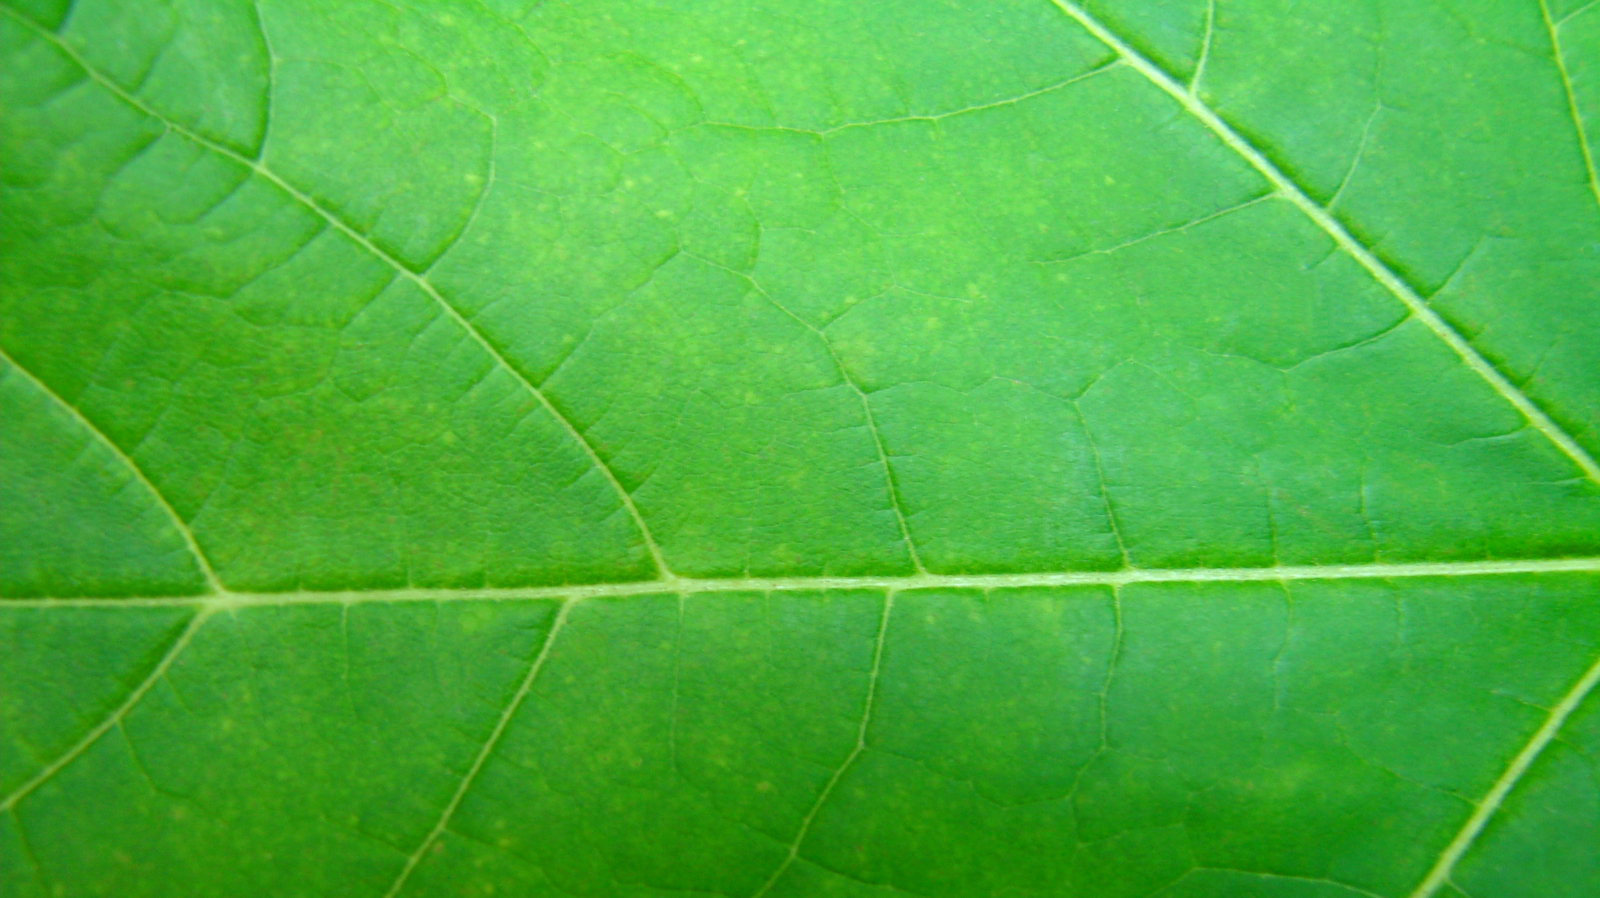
\includegraphics[scale=0.264]{images/title.jpg}\protect\footnotemark{}
\end{textblock}
\footnotetext{Quelle: \url{http://www.freeimages.com/photo/1358335}}

\begin{textblock}{154} (28,135)
    \begin{picture}(150,2)
        \put(0,0){\color{bfhgrey}\rule{150mm}{2mm}}
    \end{picture}
\end{textblock}
\color{black}

\begin{flushleft}

\vspace*{120mm}

\fontsize{26pt}{28pt}\selectfont
Erkennung von aktiven Konturen mittels Matlab
\vspace{3mm}

\fontsize{20pt}{22pt}\selectfont
Projektarbeit
\vspace{3mm}

\fontsize{10pt}{12pt}\selectfont
\textbf{BZG1301: Programmierung mit Matlab/Octave} \\
\vspace{3mm}

\begin{textblock}{150} (28,215)
\fontsize{10pt}{17pt}\selectfont
\begin{tabbing}
xxxxxxxxxxxxxxx\=xxxxxxxxxxxxxxxxxxxxxxxxxxxxxxxxxxxxxxxxxxxxxxx \kill
Autor:        \> Sven Osterwalder\\
Datum:        \> \versiondate\\
Betreuer:     \> Marx Stampfli\\
\end{tabbing}

\end{textblock}
\end{flushleft}

\begin{textblock}{150} (28,280)
\noindent 
\color{bfhgrey}\fontsize{9pt}{10pt}\selectfont
Berner Fachhochschule | Haute école spécialisée bernoise | Bern University of Applied Sciences
\color{black}\selectfont
\end{textblock}


\end{titlepage}
